%!TEX program = lualatex
% SPDX-License-Identifier: CC-BY-SA-4.0
\documentclass[11pt]{article}

\usepackage{iftex}
\ifLuaTeX\else
  \PackageError{vintage-latex}{This example requires LuaLaTeX}
    {Run lualatex, not pdflatex or xelatex.}
\fi

\usepackage{fontspec}
\usepackage{xcolor}
\usepackage{geometry}
\usepackage[tracking=true,protrusion=false,expansion=false]{microtype}
\usepackage{pgfplots}
\pgfplotsset{compat=1.18}

\defaultfontfeatures{Renderer=HarfBuzz}
\setmainfont{EB Garamond}[Numbers={OldStyle,Proportional}]
\definecolor{labpaper}{HTML}{F4EAD8}
\definecolor{gridink}{HTML}{B8956B}    % the sepia ruling of printed graph paper
\definecolor{printerink}{HTML}{25201B}
\pagecolor{labpaper}
\color{printerink}
\geometry{a5paper,landscape,top=14mm,bottom=14mm,left=16mm,right=16mm}
\pagestyle{empty}

\begin{document}

\begin{center}
  {\small\textls[110]{\textsc{Experiment XIV}}}\par
  \vspace{.25em}
  {\large Curve of Cooling of a Brass Ball in Still Air}\par
\end{center}

\vspace{.3em}

\begin{center}
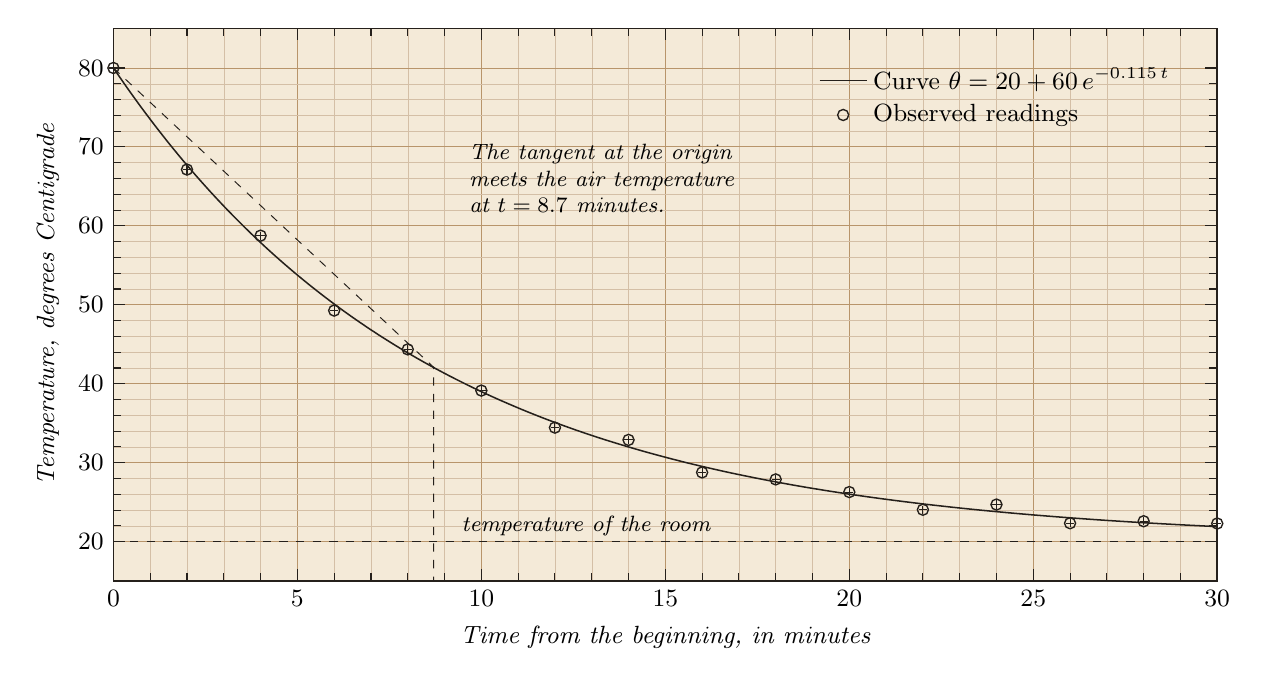
\begin{tikzpicture}
\begin{axis}[
  width=15.6cm, height=8.6cm,
  xmin=0, xmax=30, ymin=15, ymax=85,
  % Printed graph paper: a fine sepia ruling with a heavier line every fifth.
  axis background/.style={fill=labpaper},
  grid=both,
  minor tick num=4,
  major grid style={gridink,line width=.32pt},
  minor grid style={gridink!60,line width=.16pt},
  % Old chart conventions: ticks drawn inward, no tick on the far axes.
  axis line style={printerink,line width=.6pt},
  tick align=inside,
  tick style={printerink,line width=.4pt},
  xtick={0,5,...,30}, ytick={20,30,...,80},
  tick label style={font=\small},
  xlabel={\itshape Time from the beginning, in minutes},
  ylabel={\itshape Temperature, degrees Centigrade},
  label style={font=\small},
  legend style={font=\small,draw=none,fill=none,at={(.97,.95)},anchor=north east},
  legend cell align=left,
  clip=false
]
  % A smooth curve of the kind that was drawn through the points by hand.
  \addplot[printerink,line width=.55pt,smooth,samples=80,domain=0:30]
    {20 + 60*exp(-0.115*x)};
  % Readings every two minutes. The deterministic ripple stands in for the
  % scatter that a thermometer read by eye would show; nothing is random.
  \addplot[only marks,mark=o,mark size=2pt,
           mark options={printerink,line width=.5pt},
           samples at={0,2,...,30}]
    {20 + 60*exp(-0.115*x) + 0.9*sin(deg(1.9*x))};
  \addplot[only marks,mark=+,mark size=1.5pt,
           mark options={printerink,line width=.4pt},
           samples at={0,2,...,30}]
    {20 + 60*exp(-0.115*x) + 0.9*sin(deg(1.9*x))};
  \legend{Curve $\theta = 20 + 60\,e^{-0.115\,t}$, Observed readings}

  % Construction for the time constant, added as a marginal remark.
  \draw[printerink,line width=.35pt,dashed]
    (axis cs:0,80) -- (axis cs:8.7,42.1) -- (axis cs:8.7,15);
  \node[font=\footnotesize\itshape,anchor=west,align=left]
    at (axis cs:9.4,66) {The tangent at the origin\\
                          meets the air temperature\\
                          at $t = 8.7$ minutes.};
  \draw[printerink,line width=.3pt,dashed] (axis cs:0,20) -- (axis cs:30,20);
  \node[font=\footnotesize\itshape,anchor=south west,inner sep=2pt]
    at (axis cs:9.3,20) {temperature of the room};
\end{axis}
\end{tikzpicture}
\end{center}

\vspace{.2em}
\footnotesize\noindent
Ruled graph paper, inward ticks, an open-circle-and-cross plotting symbol, and
an italic caption in the margin of the chart are separate conventions of
early laboratory charts. The curve and the readings are computed from a single
expression, so the figure regenerates exactly on every compilation.

\end{document}
